% !TEX root = ./ECEN-629 - Homework 1 - Brody Jordan.tex

\documentclass[11pt]{article}

\usepackage[
    assignmentDueDate={September 16, 2025 at 12:45 pm}
]{C:/Users/bljor/Sync/Courses/assignment}

\usepackage{amsmath}
\usepackage{multirow}
\usepackage{empheq}
\usepackage{tikz}
\usepackage{tikz-3dplot}
\usepackage{subcaption}

\newcommand*\ruleline[1]{\par\noindent\raisebox{.8ex}{\makebox[\linewidth]{\hrulefill\hspace{1ex}\raisebox{-.8ex}{#1}\hspace{1ex}\hrulefill}}}


% Load TikZ libraries for advanced arrows and positioning
\usetikzlibrary{arrows.meta, positioning}

% Define a professional color palette for clarity and aesthetics
\definecolor{myblue}{RGB}{55, 126, 184}
\definecolor{myorange}{RGB}{255, 127, 0}
\definecolor{mygray}{RGB}{150, 150, 150}
\DeclareMathOperator{\tr}{tr}
\renewcommand{\norm}[1]{\left\lVert#1\right\rVert}

\begin{document}
\makeAssignmentTitle

% -- PROBLEM 1 --
\begin{homeworkProblem}

Compute the norm of the following vector $x = (-100, -99, -98, \ldots, 99, 100)^T$.

\begin{enumerate}[label=(\alph*), topsep=5pt]
    \item $\ell_1$ norm;
    \item $\ell_\infty$ norm;
    \item $\ell_2$ norm.
\end{enumerate} \vspace{1\baselineskip}

\solution

We have the definition of a norm as 
\[
    \norm{x}_p = \left( \sum_{i=1}^{n} |x_i|^p \right)^{\!\!1/p}
\]
Then for each part we have:
\begin{align*}
    \ell_1: \norm{x}_1 &= |-100| + |-99| + \ldots + |99| + |100| \\
    &= 2(1 + 2 + \ldots + 99 + 100) \\
    &= 2 \cdot \frac{100 \cdot 101}{2} \\
    &= 10100 \\\\
    \ell_\infty: \norm{x}_\infty &=  \max\{x\} \\
    &= 100 \\\\
    \ell_2: \norm{x}_2 &= \sqrt{(-100)^2 + (-99)^2 + \ldots + (99)^2 + (100)^2} \\
    &= \sqrt{2(1^2 + 2^2 + \ldots + 99^2 + 100^2)} \\
    &= \sqrt{2 \cdot \frac{100 \cdot 101 \cdot 201}{6}} \\
    &= \sqrt{676700} \\
    &\approx 822.62
\end{align*}

\end{homeworkProblem}

\pagebreak

% -- PROBLEM 2 --
\begin{homeworkProblem}

For a quadratic function $f(x) = x^T P x + q^T x + r$ where $P$ is not necessarily symmetric, show that the gradient 
is $\nabla f(x) = (P + P^T) x + q$. Find the Hessian of the function. Provide details in your proofs. \vspace{1\baselineskip}

\solution

I start be decomposing $f(x)$ into summations:
\[
    f(x) = \sum_{i=1}^m \sum_{j=1}^m P_{ij} x_i x_j + \sum_{i=1}^m q_i x_i + r
\]
Then we find the partials of the first term:
\begin{align*}
    \frac{\partial}{\partial x_k} f(x) &= \frac{\partial}{\partial x_k} \left( \sum_{i=1}^m \sum_{j=1}^m P_{ij} x_i x_j \right) 
    = \sum_{i=1}^m \sum_{j=1}^m \frac{\partial}{\partial x_k} (P_{ij} x_i x_j) \\
    &= \sum_{i=1}^m P_{kj} x_j + \sum_{j=1}^m P_{ik} x_i
\end{align*}
And the second term:
\[
    \frac{\partial}{\partial x_k} \left( \sum_{i=1}^m q_i x_i + r \right) = q_k
\]
The final term $r$ is constant, so its derivative is zero. \\

Now we can combine these indexed derivatives to get the gradient:
\begin{align*}
    \nabla f(x) = (P + P^T)x + q
\end{align*}
Now the Hessian of $f(x)$ is found by taking the partials of the gradient we just found:
\begin{align*}
    \mathbf{H} = \nabla^2 f(x) = P + P^T
\end{align*}
\end{homeworkProblem}

\pagebreak

% -- PROBLEM 3 --
\begin{homeworkProblem}

A matrix $A \in \mathbb{R}^{m \times n}$ can also be viewed as a vector, by stacking all its $n$ columns into a single 
length-$mn$ column. Let $x \in \mathbb{R}^m$, $y \in \mathbb{R}^n$ be two column vectors. Show that
\[
    \tr(A^T xy^T) = \left<xy^T, A\right> = x^T Ay,
\] 
where $\tr$ is the trace of the matrix. \vspace{1\baselineskip}

\solution

We know that rotation of our trace elements gives us 
\[
    \tr(A^T x y^T) = \tr(y^T A^T x)
\]
Here the product inside the trace is a $1 \times 1$ matrix, thus 
\[
    \tr(y^T A^T x) = y^T A^T x = x^T A y
\]
The inner product is defined as
\[
    \left<xy^T, A\right> = \sum_{i=1}^{m}\sum_{j=1}^{n} (xy^T)_{ij} A_{ij} = \sum_{i=1}^{m}\sum_{j=1}^{n} x_i y_j A_{ij} = x^T A y
\]
\end{homeworkProblem}
Thus both the trace of $A^T xy^T$ and the inner product $\left<xy^T, A\right>$ equal $x^T A y$.
\pagebreak

% -- PROBLEM 4 --
\begin{homeworkProblem}

Let $B \in \mathbb{R}^{n \times n}$ be a given symmetric matrix of size $n$-by-$n$. Determine if the following set is convex:
the set of all $n$-by-$n$ symmetric $A$ matrices, such that $A - B$ is positive semidefinite. If it is convex, provide your
reasoning; if not, provide a counter-example. \vspace{1\baselineskip}

\solution

Putting it in set notation, we have
\[
    C = \{A \in \mathbb{S}^{n} \mid A - B \succeq 0\}
\]
Now we know that a set is convex if 
\[
    A_1, A_2 \in C, \quad 0 \leq \theta \leq 1 \quad\implies\quad \theta A_1 + (1 - \theta) A_2 \in C
\]
Writing out the set with some $A_1, A_2 \in C$, we have
\[
    \theta A_1 + (1 - \theta) A_2 - B \succeq 0
\]
Distributing the subtraction of $B$, we have
\[
    \theta (A_1 - B) + (1 - \theta)(A_2 - B) \succeq 0
\]
Since $A_1, A_2 \in C$, we know that $A_1 - B \succeq 0$ and $A_2 - B \succeq 0$. Since this is a linear 
combination of PSD's, it is also PSD. We have now seen that $\theta A_1 + (1 - \theta) A_2 \in C$, so the set 
is convex.

\end{homeworkProblem}

\pagebreak

% -- PROBLEM 5 --
\begin{homeworkProblem}

A set is defined as 
\[
    C = \{x \in \mathbb{R}^n \bigm\vert \norm{x-a}_2 \leq \theta \norm{x-y}_2 \text{ for all } y \in S\}
\]
where $S \subseteq \mathbb{R}^n$.
\begin{enumerate}[label=(\alph*), topsep=5pt]
    \item Determine whether the set is convex, which may depend on the value of $\theta$. For the case that it is,
    provide your reasoning; otherwise, provide a counter-example.
    \item Let $a = (1, 0)^T$ and $S = \{(-1, 0)^T, (0, -1)^T\}$. For $\theta = 2$ and $\theta = 0.5$, sketch the 
    resultant set, respectively.
\end{enumerate} \vspace{1\baselineskip}

\solution

\textbf{Part (a):} I will define two arbitray points in $C$, now $x_1, x_2 \in C$ and check for convexity. I'll use 
$\phi x_1 + (1 - \phi) x_2$ to avoid confusion with $\theta$.
\[
    \norm{\phi x_1 + (1 - \phi)x_2 - a}_2 \leq \theta \norm{\phi x_1 + (1 - \phi)x_2 - y}_2, \quad \forall y \in S
\]
Which equals
\[
    \norm{\phi (x_1 - a) + (1 - \phi)(x_2 - a)}_2 \leq \theta \norm{\phi (x_1 - y) + (1 - \phi)(x_2 - y)}_2, \quad \forall y \in S
\]
The value of $\theta$ determines the size and shape of the set. \\

\textbf{Part (b):} For $\theta = 0.5$, the set is defined as s
\[ 
    \{x \in \mathbb{R}^n \bigm\vert \norm{x-(1,0)^T}_2 \leq 0.5 \norm{x-y}_2 \text{ for all } y \in S\}
\]
Which simplifies to the regions $(x_1 - 1)^2 + x_2^2 \leq 0.25((x_1 + 1)^2 + x_2^2)$ and $(x_1 - 1)^2 + x_2^2 \leq 0.25(x_1^2 + (x_2 + 1)^2)$.
Plotting those regions

\begin{figure}[hbpt!]
    \centering
    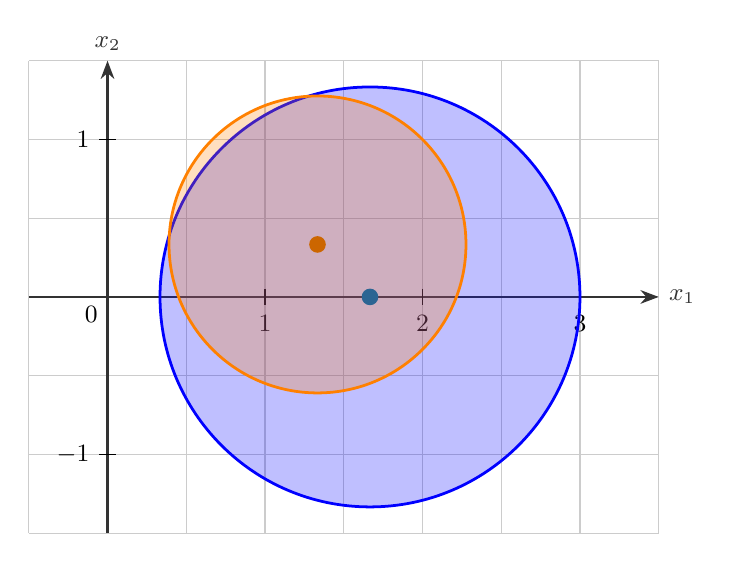
\begin{tikzpicture}[scale=2,
        % Set global font size for consistency
        font=\small,
        % Define reusable styles for different elements of the plot
        axis/.style={-Stealth, thick, black!80},
        grid/.style={thin, black!20},
        region1/.style={draw=blue, fill=blue, fill opacity=0.25, line width=1pt},
        region2/.style={draw=orange, fill=orange, fill opacity=0.25, line width=1pt},
        label/.style={font=\footnotesize}
    ]

    \draw[grid, step=0.5] (-0.5, -1.5) grid (3.5, 1.5);
    \draw[axis] (-0.5, 0) -- (3.5, 0) node[right] {$x_1$};
    \draw[axis] (0, -1.5) -- (0, 1.5) node[above] {$x_2$};

    % Axis ticks and labels
    \foreach \x in {1, 2, 3} {
        \draw (\x, 1.5pt) -- (\x, -1.5pt) node[below] {$\x$};
    }
    \foreach \y in {-1, 1} {
        \draw (1.5pt, \y) -- (-1.5pt, \y) node[left] {$\y$};
    }
    \node[below left] at (0,0) {$0$};

    \filldraw[region1] ({5/3}, 0) circle ({4/3});
    \filldraw[region2] ({4/3}, {1/3}) circle ({sqrt(8)/3});

    \fill[myblue!80!black] ({5/3}, 0) circle (1.5pt);
    \fill[myorange!80!black] ({4/3}, {1/3}) circle (1.5pt);

    \end{tikzpicture}
    \vspace{-0.5\baselineskip}
    \caption{Set for $\theta = 0.5$}
\end{figure}

\newpage

For $\theta = 2$, the set is defined as
\[ 
    \{x \in \mathbb{R}^n \bigm\vert \norm{x-(1,0)^T}_2 \leq 2 \norm{x-y}_2 \text{ for all } y \in S\}
\]
Which simplifies to the regions $(x_1 - 1)^2 + x_2^2 \leq 4((x_1 + 1)^2 + x_2^2)$ and $(x_1 - 1)^2 + x_2^2 \leq 4(x_1^2 + (x_2 + 1)^2)$. \\

Plotting those regions

\begin{figure}[hbpt!]
    \centering
    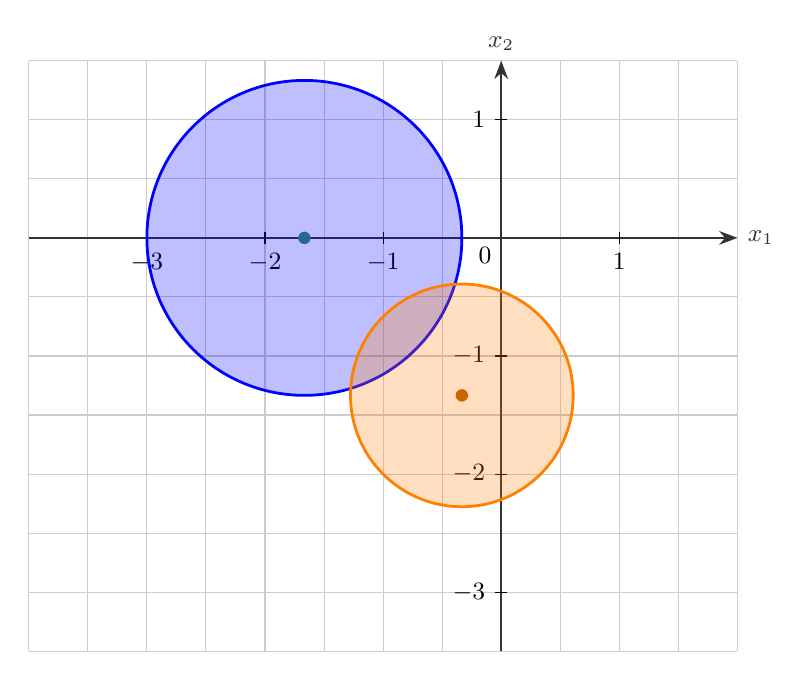
\begin{tikzpicture}[scale=1.5,
            % Set global font size for consistency
            font=\small,
            % Define reusable styles for different elements of the plot
            axis/.style={-Stealth, thick, black!80},
            grid/.style={thin, black!20},
            region1/.style={draw=blue, fill=blue, fill opacity=0.25, line width=1pt},
            region2/.style={draw=orange, fill=orange, fill opacity=0.25, line width=1pt}
        ]

        \draw[grid, step=0.5] (-4, -3.5) grid (2, 1.5);
        \draw[axis] (-4, 0) -- (2, 0) node[right] {$x_1$};
        \draw[axis] (0, -3.5) -- (0, 1.5) node[above] {$x_2$};

        \foreach \x in {-3, -2, -1, 1} {
            \draw (\x, 1.5pt) -- (\x, -1.5pt) node[below] {$\x$};
        }
        \foreach \y in {-3, -2, -1, 1} {
            \draw (1.5pt, \y) -- (-1.5pt, \y) node[left] {$\y$};
        }
        \node[below left] at (0,0) {$0$};

        \filldraw[region1] ({-5/3}, 0) circle ({4/3});
        \filldraw[region2] ({-1/3}, {-4/3}) circle ({sqrt(8)/3});

        % Mark the centers of the circular boundaries
        \fill[myblue!80!black] ({-5/3}, 0) circle (1.5pt);
        \fill[myorange!80!black] ({-1/3}, {-4/3}) circle (1.5pt);

\end{tikzpicture}
    \vspace{-0.5\baselineskip}
    \caption{Set for $\theta = 2$}
\end{figure}

\end{homeworkProblem}

\pagebreak

% -- PROBLEM 6 --
\begin{homeworkProblem}

\begin{enumerate}[label=(\alph*), topsep=0pt, itemsep=2pt]
    \item Show that if $S_1$ and $S_2$ are convex set in $\mathbb{R}^n$, then the set sum
    \[
        S \triangleq \{x_1 + x_2 \bigm\vert x_1 \in S_1, \, x_2 \in S_2\}
    \] is also convex.
    \item Let $S_1 = \{(-1, -1)^T\}$ and $S_2 = \{(2, 2)^T + u \bigm\vert \norm{u} \leq 1\}$. What is their set sum?
    \item Show that if $S_1$ and $S_2$ are convex set in $\mathbb{R}^n$, then the inverse sum
    \[
        S \triangleq \bigcup_{1 \geq \lambda \geq 0} \{\lambda S_1 \, \cap \, (1 - \lambda)S_2\}
    \] is also convex, where $\lambda S_j = \{\lambda x_j \bigm\vert x_j \in S_j\}, \, j = 1, 2$.
    \item Let $S_1 = \{(1, 1)^T\}$ and $S_2 = \{(2, 2)^T + u \bigm\vert \norm{u} \leq 1\}$. What is their inverse sum?
\end{enumerate} \vspace{1\baselineskip}

\solution

\textbf{Part (a):} Similar to above, we choose two arbitray points in $S$
\[  
    a = x_1 + x_2, \quad b = y_1 + y_2, \quad x_1, y_1 \in S_1, \quad x_2, y_2 \in S_2
\]
and check if they satisfy the conditions of a convex set
\begin{align*}
    \theta a + (1 - \theta) b &= \theta (x_1 + x_2) + (1 - \theta)(y_1 + y_2) \\
    &= \underbrace{\theta x_1 + (1 - \theta) y_1}_{\in S_1} + \underbrace{\theta x_2 + (1 - \theta) y_2}_{\in S_2}
\end{align*}
So this is a sum of terms $x_1 + x_2$ where $x_1 \in S_1$ and $x_2 \in S_2$, so $\theta a + (1 - \theta) b \in S$. 
Thus, $S$ is a convex set. \\

\textbf{Part (b):} The set sum of $S_1$ and $S_2$ is
\begin{align*}
    S_1 + S_2 & = \{(-1, -1)^T + (2, 2)^T + u \bigm\vert \norm{u} \leq 1\} \\
    & = \{(1, 1)^T + u \bigm\vert \norm{u} \leq 1\} 
\end{align*}
Which is a circle of radius 1 centered at (1, 1). \\

\textbf{Part (c):} We choose two arbitray points $x, y \in S$ \\

\textbf{Part (d):} 

\end{homeworkProblem}

\pagebreak

% -- PROBLEM 7 --
\begin{homeworkProblem}

It is known that one halfspace contains another in the following form
\[
    \{x \bigm\vert a^T x \leq b\} \subseteq \{x \bigm\vert c \cdot a^T x \leq \tilde{b}\}.
\] Provide the conditions that the parameters $c$, $b$, and $\tilde{b}$ must satisfy. Are these conditions also sufficient for the
containment relation between these two halfspaces? \vspace{1\baselineskip}

\solution

For the first set to be a subset of the second, any $x$ that satisfies $a^T x \leq b$ must also satisfy $c \cdot a^T x \leq \tilde{b}$. \\

If $c < 0$, then $x$ must satisfy
\begin{equation*}
\begin{cases}
    a^T x \leq b \\
    c \cdot a^T x \leq \tilde{b}
\end{cases}
\implies
\begin{cases}
    a^T x \leq b \\
    a^T x \geq \tilde{b}/c
\end{cases}
\end{equation*}
Which presents a contradiction, so $c \geq 0$. \\

For $c = 0$, we have
\begin{equation*}
\begin{cases}
    a^T x \leq b \\
    0 \leq \tilde{b}
\end{cases}
\end{equation*}
Which is valid when $\tilde{b} \geq 0$. \\

For $c > 0$
\begin{equation*}
\begin{cases}
    a^T x \leq b \\
    c \cdot a^T x \leq \tilde{b}
\end{cases}
\end{equation*}
Which requires that $b \leq \tilde{b}/c$. \\

\end{homeworkProblem}

\pagebreak

% -- PROBLEM 8 --
\begin{homeworkProblem}

For a pair of given sets $C, D \subseteq \mathbb{R}^n$, consider the following set
\[
    S = \{(a, b) \in \mathbb{R}^{n + 1} \bigm\vert a^T x \leq b \text{ for all } x \in C, \, a^T x \geq b \text{ for all } x \in D\}.
\] Prove that the set $S$ is convex. \vspace{1\baselineskip}

\solution

Choosing two arbitrary points in $S$, we have
\[
    x = (a_1, b_1), \quad y = (a_2, b_2)
\]
and applying it to our convex definition
\[
    \theta x + (1 - \theta) y = (\theta a_1 + (1 - \theta) a_2, \, \theta b_1 + (1 - \theta) b_2)
\]
Now to see if this is in $S$, we check the two conditions, starting with the first
\[
    (\theta a_1 + (1 - \theta) a_2)^T x = \theta a_1^T x + (1-\theta) a_2^T x \leq \theta b_1 + (1 - \theta) b_2, \quad \forall x \in C
\]
and then the second
\[
    (\theta a_1 + (1 - \theta) a_2)^T x = \theta a_1^T x + (1-\theta) a_2^T x \geq \theta b_1 + (1 - \theta) b_2, \quad \forall x \in D
\]
Since both of these conditions hold by the set definition, the set $S$ is convex.

\end{homeworkProblem}

\pagebreak

% -- PROBLEM 9 --
\begin{homeworkProblem}

Let $C = \{X \in \mathbb{R}^{n \times n} \bigm\vert a^T X a \geq 0, \, \forall a \in \mathbb{R}^n \}$. Determine whether the set
\[
    \mathcal{S} = \{A \in \mathbb{R}^{n \times n} \bigm\vert A - M \in C \}
\]
is convex, where $M \in C$ is a fixed matrix. Provide justification or a counterexample. Note that usually the definition of a 
matrix being positive-definite requires the matrix to be symmetric, but this problem removes that condition. \vspace{1\baselineskip}

\solution

Again choose two arbitrary points in $\mathcal{S}$
\[
    A_1, A_2 \in \mathcal{S}
\]
and check the convex condition
\[
    \theta A_1 + (1 - \theta) A_2 - M \in C
\]
Distributing the subtraction of $M$, we have
\[
    \theta (A_1 - M) + (1 - \theta)(A_2 - M) \in C
\]
Now this new matrix is in $C$ if 
\[
    a^T(\theta(A_1 - M) + (1 - \theta)(A_2 - M)) a \geq 0 
\]
Which becomes
\[
    a^T (\theta(A_1 - M)) a + a^T((1 - \theta)(A_2 - M)) a \geq 0
\]
Since $A_1, A_2 \in \mathcal{S}$, we know that $A_1 - M \in C$ and $A_2 - M \in C$, so these terms are $\geq 0$. Set $\mathcal{S}$ satisfies the convex conditions, so it is convex.

\end{homeworkProblem}

\pagebreak

% -- PROBLEM 10 --
\begin{homeworkProblem}

Plot the norm balls of radius $r = 1$ for the following norm in $\mathbb{R}^2$ and $\mathbb{R}^3$:

\begin{enumerate}[label=(\alph*), topsep=5pt]
    \item $\ell_1$ norm;
    \item $\ell_\infty$ norm;
    \item $\ell_2$ norm.
\end{enumerate} \vspace{1\baselineskip}

\solution

\ruleline{$\mathbb{R}^2$} \\

\begin{figure}[htbp!]
\centering
    \begin{subfigure}[b]{0.3\textwidth}
        \centering
        \begin{tikzpicture}[scale=1.2]
            \begin{axis}
            \draw[step=0.5,gray!30] (-1.5,-1.5) grid (1.5,1.5);
            \draw[->] (-1.5,0) -- (1.5,0) node[right] {$x_1$};
            \draw[->] (0,-1.5) -- (0,1.5) node[above] {$x_2$};
            
            \draw[thick, red, fill=red!20] (1,0) -- (0,1) -- (-1,0) -- (0,-1) -- cycle;

        \end{tikzpicture}
        \caption{$\ell_1$ norm}
    \end{subfigure}
    \hfill
    \begin{subfigure}[b]{0.3\textwidth}
        \centering
        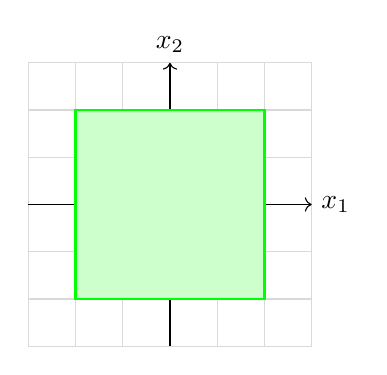
\begin{tikzpicture}[scale=1.2]
            % Grid and axes

            \draw[step=0.5,gray!30] (-1.5,-1.5) grid (1.5,1.5);
            \draw[->] (-1.5,0) -- (1.5,0) node[right] {$x_1$};
            \draw[->] (0,-1.5) -- (0,1.5) node[above] {$x_2$};
            
            \draw[thick, green, fill=green!20] (-1,-1) rectangle (1,1);

        \end{tikzpicture}
        \caption{$\ell_\infty$ norm}
    \end{subfigure}
    \hfill
    \begin{subfigure}[b]{0.3\textwidth}
        \centering
        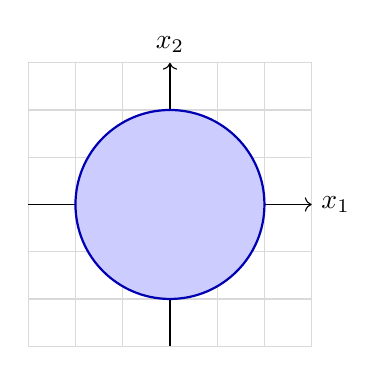
\begin{tikzpicture}[scale=1.2]
            \draw[step=0.5,gray!30] (-1.5,-1.5) grid (1.5,1.5);
            \draw[->] (-1.5,0) -- (1.5,0) node[right] {$x_1$};
            \draw[->] (0,-1.5) -- (0,1.5) node[above] {$x_2$};
            
            \draw[thick, blue!70!black, fill=blue!20] (0,0) circle (1);

        \end{tikzpicture}
        \caption{$\ell_2$ norm}
    \end{subfigure}
    \caption{Norm balls in $\mathbb{R}^2$}
\end{figure}

\vspace{1cm}


\ruleline{$\mathbb{R}^3$} 
\vspace{1\baselineskip}
\begin{figure}[htbp!]
\centering
    \begin{subfigure}[b]{0.3\textwidth}
        \centering
        \tdplotsetmaincoords{70}{110}
        \begin{tikzpicture}[scale=1.0,tdplot_main_coords]
            % Axes
            \draw[->] (-2,0,0) -- (2,0,0) node[anchor=north east]{$x_1$};
            \draw[->] (0,-2,0) -- (0,2,0) node[anchor=north west]{$x_2$};
            \draw[->] (0,0,-2) -- (0,0,2) node[anchor=south]{$x_3$};
            
            % L1 norm ball (octahedron)
            % Front faces
            \draw[thick, red, fill=red!20, opacity=0.7] (1,0,0) -- (0,1,0) -- (0,0,1) -- cycle;
            \draw[thick, red, fill=red!15, opacity=0.7] (1,0,0) -- (0,-1,0) -- (0,0,1) -- cycle;
            \draw[thick, red, fill=red!25, opacity=0.7] (-1,0,0) -- (0,1,0) -- (0,0,1) -- cycle;
            \draw[thick, red, fill=red!10, opacity=0.7] (-1,0,0) -- (0,-1,0) -- (0,0,1) -- cycle;
            
            % Bottom faces
            \draw[thick, red, fill=red!30, opacity=0.7] (1,0,0) -- (0,1,0) -- (0,0,-1) -- cycle;
            \draw[thick, red, fill=red!20, opacity=0.7] (1,0,0) -- (0,-1,0) -- (0,0,-1) -- cycle;
            \draw[thick, red, fill=red!35, opacity=0.7] (-1,0,0) -- (0,1,0) -- (0,0,-1) -- cycle;
            \draw[thick, red, fill=red!15, opacity=0.7] (-1,0,0) -- (0,-1,0) -- (0,0,-1) -- cycle;
        \end{tikzpicture}
        \caption{$\ell_1$ norm}
    \end{subfigure}
    \hfill
    \begin{subfigure}[b]{0.3\textwidth}
        \centering
        \tdplotsetmaincoords{70}{110}
        \begin{tikzpicture}[scale=1.0,tdplot_main_coords]
            % Axes
            \draw[->] (-2,0,0) -- (2,0,0) node[anchor=north east]{$x_1$};
            \draw[->] (0,-2,0) -- (0,2,0) node[anchor=north west]{$x_2$};
            \draw[->] (0,0,-2) -- (0,0,2) node[anchor=south]{$x_3$};

            \draw[thick, green] (-1,-1,-1) -- (1,-1,-1) -- (1,1,-1) -- (-1,1,-1) -- cycle;
            \draw[thick, green] (-1,-1,1) -- (1,-1,1) -- (1,1,1) -- (-1,1,1) -- cycle;
            
            % Connecting edges
            \draw[thick, green] (-1,-1,-1) -- (-1,-1,1);
            \draw[thick, green] (1,-1,-1) -- (1,-1,1);
            \draw[thick, green] (1,1,-1) -- (1,1,1);
            \draw[thick, green] (-1,1,-1) -- (-1,1,1);
            
            % Front faces (with fill)
            \draw[thick, green, fill=green!15, opacity=0.7] (-1,1,-1) -- (-1,1,1) -- (1,1,1) -- (1,1,-1) -- cycle;
            \draw[thick, green, fill=green!20, opacity=0.7] (-1,-1,-1) -- (1,-1,-1) -- (1,-1,1) -- (-1,-1,1) -- cycle;
            \draw[thick, green, fill=green!25, opacity=0.7] (1,-1,-1) -- (1,1,-1) -- (1,1,1) -- (1,-1,1) -- cycle;
            \draw[thick, green, fill=green!30, opacity=0.7] (-1,-1,1) -- (1,-1,1) -- (1,1,1) -- (-1,1,1) -- cycle;
        \end{tikzpicture}
        \caption{$\ell_\infty$ norm}
    \end{subfigure}
    \hfill
    \begin{subfigure}[b]{0.3\textwidth}
        \centering
        \tdplotsetmaincoords{70}{110}
        \begin{tikzpicture}[scale=1.0,tdplot_main_coords]
            % Axes
            \draw[->] (-2,0,0) -- (2,0,0) node[anchor=north east]{$x_1$};
            \draw[->] (0,-2,0) -- (0,2,0) node[anchor=north west]{$x_2$};
            \draw[->] (0,0,-2) -- (0,0,2) node[anchor=south]{$x_3$};
            
            % L2 norm ball (sphere) - using multiple circles
            % Horizontal circles at different z levels
            \foreach \z in {-0.8,-0.4,0,0.4,0.8} {
                \pgfmathsetmacro{\radius}{sqrt(1-\z*\z)}
                \draw[blue!70!black, opacity=0.3] (0,0,\z) circle (\radius);
            }
            
            % Vertical circles
            \tdplotsetrotatedcoords{0}{90}{0}
            \draw[thick, blue!70!black, fill=blue!20, opacity=0.4, tdplot_rotated_coords] (0,0,0) circle (1);
            \tdplotsetrotatedcoords{90}{90}{0}
            \draw[thick, blue!70!black, fill=blue!15, opacity=0.4, tdplot_rotated_coords] (0,0,0) circle (1);
            
            % Main outline circle
            \draw[thick, blue!70!black] (0,0,0) circle (1);
        \end{tikzpicture}
        \caption{$\ell_2$ norm}
    \end{subfigure}
    \caption{Norm balls in $\mathbb{R}^3$}
\end{figure}

\end{homeworkProblem}

\end{document}